%!TEX program = xelatex
% 完整编译方法 1: pdflatex -> bibtex -> pdflatex -> pdflatex
% 完整编译方法 2: xelatex -> bibtex -> xelatex -> xelatex
\documentclass[lang=cn,11pt,numbers, a4paper]{elegantpaper}

\title{ElegantPaper: 一个优美的 \LaTeX{} 工作论文模板}
\author{Ethan DENG \\ Fudan University \and Dongsheng DENG \\ PA Technology}
\institute{\href{https://elegantlatex.org/}{Elegant\LaTeX{} 项目组}}

\version{0.08}
\date{\zhtoday}

\begin{document}

\maketitle

\begin{abstract}
本文为 \href{https://github.com/ElegantLaTeX/ElegantPaper/}{ElegantPaper} 的说明文档(中文)。此模板基于 \LaTeX{} 的 article 类,专为工作论文写作而设计。设计这个模板的初衷是让作者不用关心工作论文的格式,专心写作,从而有更加舒适,简便的写作体验。如果你有其他问题、建议或者报告 bug,可以在 \href{https://github.com/ElegantLaTeX/ElegantPaper/issues}{ElegantPaper/issues} 留言。如果你想了解更多由 Elegant\LaTeX{} 项目组设计的模板,请访问 \href{https://github.com/ElegantLaTeX/}{https://github.com/ElegantLaTeX/}。
\keywords{Elegant\LaTeX{},工作论文,模板}
\end{abstract}


\section{模板介绍}

此模板基于 \LaTeX{} 的标准文类 article 设计,也即意味着你可以把 article 文类的选项传递给本模板,比如 \lstinline{a4paper, 11pt} 等等。本模板支持 \hologo{pdfLaTeX} 和 \hologo{XeLaTeX} 编译。

\begin{lstlisting}
\documentclass[a4paper,11pt]{elegantpaper}
\end{lstlisting}

\textbf{注意}:Elegant\LaTeX{} 系列模板已经全部上传至 \href{https://www.overleaf.com}{Overleaf} 上,用户可以在线使用 \href{https://www.overleaf.com/latex/templates/elegantpaper-template/yzghrqjhmmmr}{ElegantPaper}。
  
\subsection{全局选项}
此模板定义了一个语言选项 \lstinline{lang},可以选择英文模式 \lstinline{lang=en}(默认)或者中文模式 \lstinline{lang=cn}。当选择中文模式时,图表的标题引导词以及参考文献,定理引导词等信息会变成中文。你可以通过下面两种方式来选择语言模式:
\begin{lstlisting}
\documentclass[lang=cn]{elegantpaper} % or
\documentclass{cn}{elegantpaper} 
\end{lstlisting}

\textbf{注意:} 英文模式下,由于没有添加中文宏包,无法输入中文。如果需要输入中文,可以通过在导言区引入中文宏包 \lstinline{ctex} 或者加入 \lstinline{xeCJK} 宏包后自行设置字体。 
\begin{lstlisting}
\usepackage[UTF8,scheme=plain]{ctex}
\end{lstlisting}

\subsection{英文与数学字体}

本模板使用 \lstinline{newtxtext} 和 \lstinline{newtxmath} 分别设置全文的英文文本字体和数学字体。数学字体的效果如下:
\begin{equation}
(a+3b)^{n} = \sum_{k=0}^{n} C_{n}^{k} a^{n-k} (3b)^k\label{eq:binom}
\end{equation}

\subsection{自定义命令}
此模板并没有修改任何默认的 \LaTeX{} 命令或者环境。另外,我自定义了 4 个命令:
\begin{enumerate}
    \item \lstinline{\email}:创建邮箱地址的链接,比如 \email{ddswhu@outlook.com};
    \item \lstinline{\figref}:用法和 \lstinline{\ref} 类似,但是会在插图的标题前添加 <\textbf{图 n}> ;
    \item \lstinline{\tabref}:用法和 \lstinline{\ref} 类似,但是会在表格的标题前添加 <\textbf{表 n}>;
    \item \lstinline{\keywords}:为摘要环境添加关键词。
\end{enumerate}

\subsection{列表环境}
你可以使用列表环境(\lstinline{itemize}、\lstinline{enumerate}、\lstinline{description}),示例如下:\\[2ex]
\begin{minipage}[c]{0.59\linewidth}
\begin{lstlisting}
\begin{itemize}
   \item Routing and resource discovery;
   \item Resilient and scalable networks; 
   \item Distributed storage and search.
\end{itemize}
\end{lstlisting}
\end{minipage}
\begin{minipage}[c]{0.4\linewidth}
\begin{itemize}
   \item Routing and resource discovery;
   \item Resilient and scalable networks;
   \item Distributed storage and search.
\end{itemize}
\end{minipage}


\subsection{插图}
插图的命令和以前一样,也是使用 \lstinline{figure} 环境。\figref{fig:scatter} 显示了插图的效果。你可以把你的图放到当前工作目录的如下子目录下 (\lstinline{./image/}, \lstinline{./img/}, \lstinline{./figure/}, \lstinline{./fig/})。
\begin{lstlisting}
\begin{figure}[htbp]
	\centering
	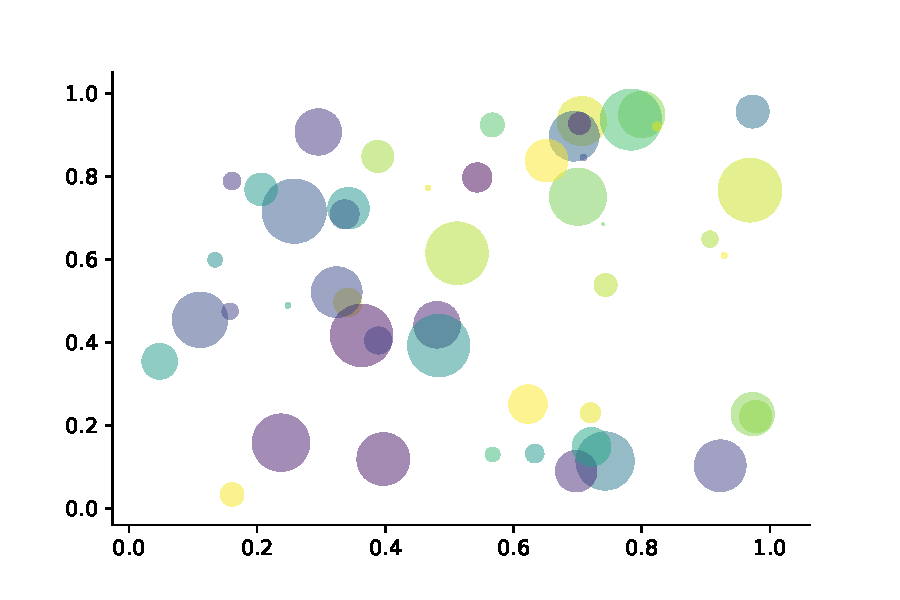
\includegraphics[width=0.6\textwidth]{scatter.pdf}
	\caption{Scatter Plot Example \label{fig:scatter}}
\end{figure}
\end{lstlisting}
\begin{figure}[htbp]
	\centering
	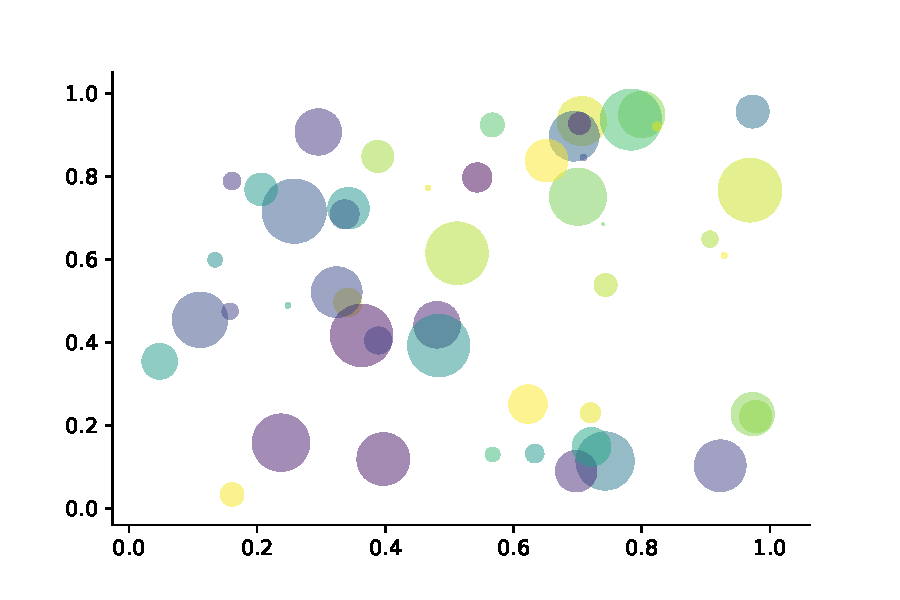
\includegraphics[width=0.6\textwidth]{scatter.pdf}
	\caption{Scatter Plot Example \label{fig:scatter}}
\end{figure}

\subsection{表格}
建议使用 \lstinline{booktabs} 宏包制作表格,该宏包有三个命令 \lstinline{\toprule}、\lstinline{\midrule} 和 \lstinline[breaklines]{\bottomrule} 能方便你制作三线表。\tabref{tab:reg} 是一个示例:
\begin{lstlisting}
\begin{table}[htbp]
  \small
  \centering
  \caption{Auto MPG and Price \label{tab:reg}}
    \begin{tabular}{lcc}
    \toprule
                    &       (1)         &        (2)      \\
    \midrule
    mpg             &    -238.90***     &      -49.51     \\
                    &     (53.08)       &      (86.16)    \\
    weight          &                   &      1.75***    \\
                    &                   &      (0.641)    \\
    constant        &     11,253***     &       1,946     \\
                    &     (1,171)       &      (3,597)    \\
    obs             &        74         &         74      \\
    $R^2$           &      0.220        &       0.293     \\
    \bottomrule
    \multicolumn{3}{l}{\scriptsize Standard errors in parentheses} \\
    \multicolumn{3}{l}{\scriptsize *** p<0.01, ** p<0.05, * p<0.1} \\
    \end{tabular}%
\end{table}%
\end{lstlisting}
\begin{table}[htbp]
  \small
  \centering
  \caption{Auto MPG and Price \label{tab:reg}}
    \begin{tabular}{lcc}
    \toprule
                    &       (1)         &        (2)      \\
    \midrule
    mpg             &    -238.90***     &      -49.51     \\
                    &     (53.08)       &      (86.16)    \\
    weight          &                   &      1.75***    \\
                    &                   &      (0.641)    \\
    constant        &     11,253***     &       1,946     \\
                    &     (1,171)       &      (3,597)   \\
    obs             &        74         &         74     \\
    $R^2$           &      0.220        &       0.293    \\
    \bottomrule
    \multicolumn{3}{l}{\scriptsize Standard errors in parentheses} \\
    \multicolumn{3}{l}{\scriptsize *** p<0.01, ** p<0.05, * p<0.1} \\
    \end{tabular}%
\end{table}%



\subsection{参考文献}
此模板使用 \hologo{BibTeX} 来生成参考文献,默认使用的文献样式(bib style)是 \lstinline{GB/T 7714-2015}\footnote{通过调用 \href{https://ctan.org/pkg/gbt7714}{\lstinline{gbt7714}} 宏包}。参考文献示例:~\cite{en3} 使用了中国一个大型的 P2P 平台(人人贷)的数据来检验男性投资者和女性投资者在投资表现上是否有显著差异。

你可以在谷歌学术,Mendeley,Endnote 中获得文献条目(bib item),然后把它们添加到 \lstinline{wpref.bib} 中。在文中引用的时候,引用它们的键值(bib key)即可。注意需要在编译的过程中添加 \hologo{BibTeX} 编译。

本模板还添加了 \lstinline{cite=numbers} 、\lstinline{cite=super} 和 \lstinline{cite=authoryear}  三个参考文献选项,用于设置参考文献格式的设置,默认为 \lstinline{super}。理工科类一般使用数字形式 \lstinline{numbers} 或者上标形式 \lstinline{super},而文科类多使用作者--年份 \lstinline{authoryear} 比较多。如果需要改为 \lstinline{cite=numbers}  或者  \lstinline{authoryear} ,可以使用
\begin{lstlisting}
\documentclass[cite=numbers]{elegantpaper} % numbers style ref style
\documentclass[numbers]{elegantpaper}

\documentclass[cite=authoryear]{elegantpaper} % author-year ref style
\documentclass[authoryear]{elegantpaper}
\end{lstlisting}

\section{常见问题 FAQ}

\begin{enumerate}[label=\arabic*).]
\item \textit{如何删除版本信息?}\\
导言区不写 \lstinline|\version{x.xx}| 即可。
\item \textit{如何删除日期?}\\
需要注意的是,与版本 \lstinline{\version} 不同的是,导言区不写或注释 \lstinline{\date} 的话,仍然会打印出当日日期,原因是 \lstinline{\date} 有默认参数。如果不需要日期的话,日期可以留空即可,也即 \lstinline|\date{}|。
\item \textit{如何获得中文日期?}\\
为了获得中文日期,必须在中文模式下\footnote{英文模式下,由于未加载中文宏包,无法输入中文。},使用 \lstinline|\date{\zhdate{2019/10/10}}|,如果需要当天的汉化日期,可以使用 \lstinline|\date{\zhtoday}|,这两个命令都来源于 \href{https://ctan.org/pkg/zhnumber}{\lstinline{zhnumber}} 宏包。
\item \textit{如何添加多个作者?}\\
在 \lstinline{\author} 里面使用 \lstinline{\and},作者单位可以用 \lstinline{\\} 换行。
\begin{lstlisting}
\author{Author A \\ Org. A \and Author B \\ Org. B }
\end{lstlisting}
\item \textit{如何添加中英文摘要?}\\
请参考 \href{https://github.com/ElegantLaTeX/ElegantPaper/issues/5}{Github::ElegantPaper/issues/5}
\end{enumerate}

\section{示例}
这是一个示例文档:
\begin{lstlisting}
\documentclass[lang=cn,a4paper,11pt]{elegantpaper}

% title information
\title{Working Paper Example}
\author{Author Name} 
\institute{Elegant\LaTeX{} Group}

\version{1.00}
\date{\today}

\begin{document}

\maketitle

\begin{abstract}
Your abstract goes here.
\keywords{keyword1, keyword2}
\end{abstract}

\section{Introduction}
The content of introduction section.

\section{Conclusion}
The content of conclusion section.

\bibliography{wpref}

\end{document}
\end{lstlisting}

\nocite{*}
\bibliography{wpref}

\end{document}
